\documentclass{article}
\usepackage{textcomp}
\usepackage[english]{babel}
\usepackage[utf8]{inputenc}
\usepackage{lmodern}
\usepackage{textcomp}
\usepackage[T1]{fontenc}
\usepackage{ucs}
\usepackage{amssymb}
\usepackage{amsmath}
\usepackage{courier}
\usepackage{graphicx}
\usepackage{a4wide}

\newcommand{\quality}[1]{q_{#1}}
\newcommand{\minfun}{\text{min}}
\newcommand{\realvec}[1]{\mathbf{#1}}
\newcommand{\norm}[1]{\left\| #1 \right\|}
\newcommand{\derivative}[2]{\frac{\partial #1}{\partial #2}}
\newcommand{\timederivative}[1]{\derivative{#1}{t}}
\newcommand{\realnumber}{\mathbb{R}}
\setcounter{secnumdepth}{2}

\author{Jonas Östlund}
\date{\today}
\title{Automatic Calibration of Nautical Instruments}

\begin{document}
\maketitle
\section{Introduction}
Properly calibrating instruments on a boat is important in order for sailors basing their decisions on sensor data to make close to optimal decisions that can help them win races. However, traditional calibration of instruments is a complicated procedure to carry out and therefore, many sailors skip it. It is therefore desirable to automate calibration in order to save time and let more sailors enjoy the benefits of properly calibrated nautical instruments.

However, automatic calibration of instruments is a difficult problem due to the many unknown parameters. Not only are the parameters of the instruments unknown, but also the local wind and current conditions. Therefore, domain knowledge is required to build a model that can lead to a well-posed optimization problem.

One such model is based on the assumption that when a manoeuver is performed and the local wind and current conditions are stable, a true wind and current estimated from improperly calibrated instruments would be unstable. Calibrating the instruments would make the estimated true wind and current to become stable. In practice, this could be implemented by minimizing the difference between true wind just before and just after a manoeuver. An approach based on this assumption is used by Team New Zealand, but it neverthless requires a substantial amount of manual labour\footnote{According to Jean-Claude Monnin}. In order to obtain a stable estimate of the calibration parameters, the data need to be fitted to several different manoeuvers that are segmented out from data. Unfortunately, manoeuvers are sparse events and plenty of recorded data may be required to obtain sufficiently many manoeuvers over which to optimize. Furthermore, a manoeuver could be triggered by a sudden change in the wind direction. For instance, a sailor might perform a tack because a wind change lead to a less favourable VMG, which would make the assumption that the wind is relatively stable at manoeuvers less valid.

\section{Problem Formulation}
In this report, we attempt to address the concerns raised in the introduction. Specifically, we base our proposed solution on the following points:
\begin{enumerate}
 \item If the true wind and current are stable when a rapid change in the velocity of the boat takes place, we would expect the estimated true wind and current from the calibration parameters to be stable as well.
 \item If it is not true that the wind and current is stable at a rapid change in the boat velocity, the local measurements should have neglible influence on the calibration.
 \item We should be able to perform calibration also on limited amounts of data, e.g. recordings from a few hours of sailing.
\end{enumerate}.

\section{Optimization}
We formulate an optimization problem where we minimize an objective function w.r.t. $X \in \realnumber^n$ calibration parameters. The estimated true wind at a given moment is given by a function $\realvec{w}: \realnumber \times \realnumber^n \rightarrow \realnumber^2$ that maps a local time and calibration parameters to a vector in a local two-dimensional coordinate system attached to the sea surface. For the current, we have a similar function $\realvec{c}: \realnumber \times \realnumber^n \rightarrow \realnumber^2$. We assume the GPS velocity vector does not depend on any calibration parameters, but only the local time: $\realvec{g}: \realnumber \rightarrow \realnumber^2$. See Fig. \ref{fig:calib} for a diagram to estimate true wind and current from sensors.
\begin{figure}
\centering
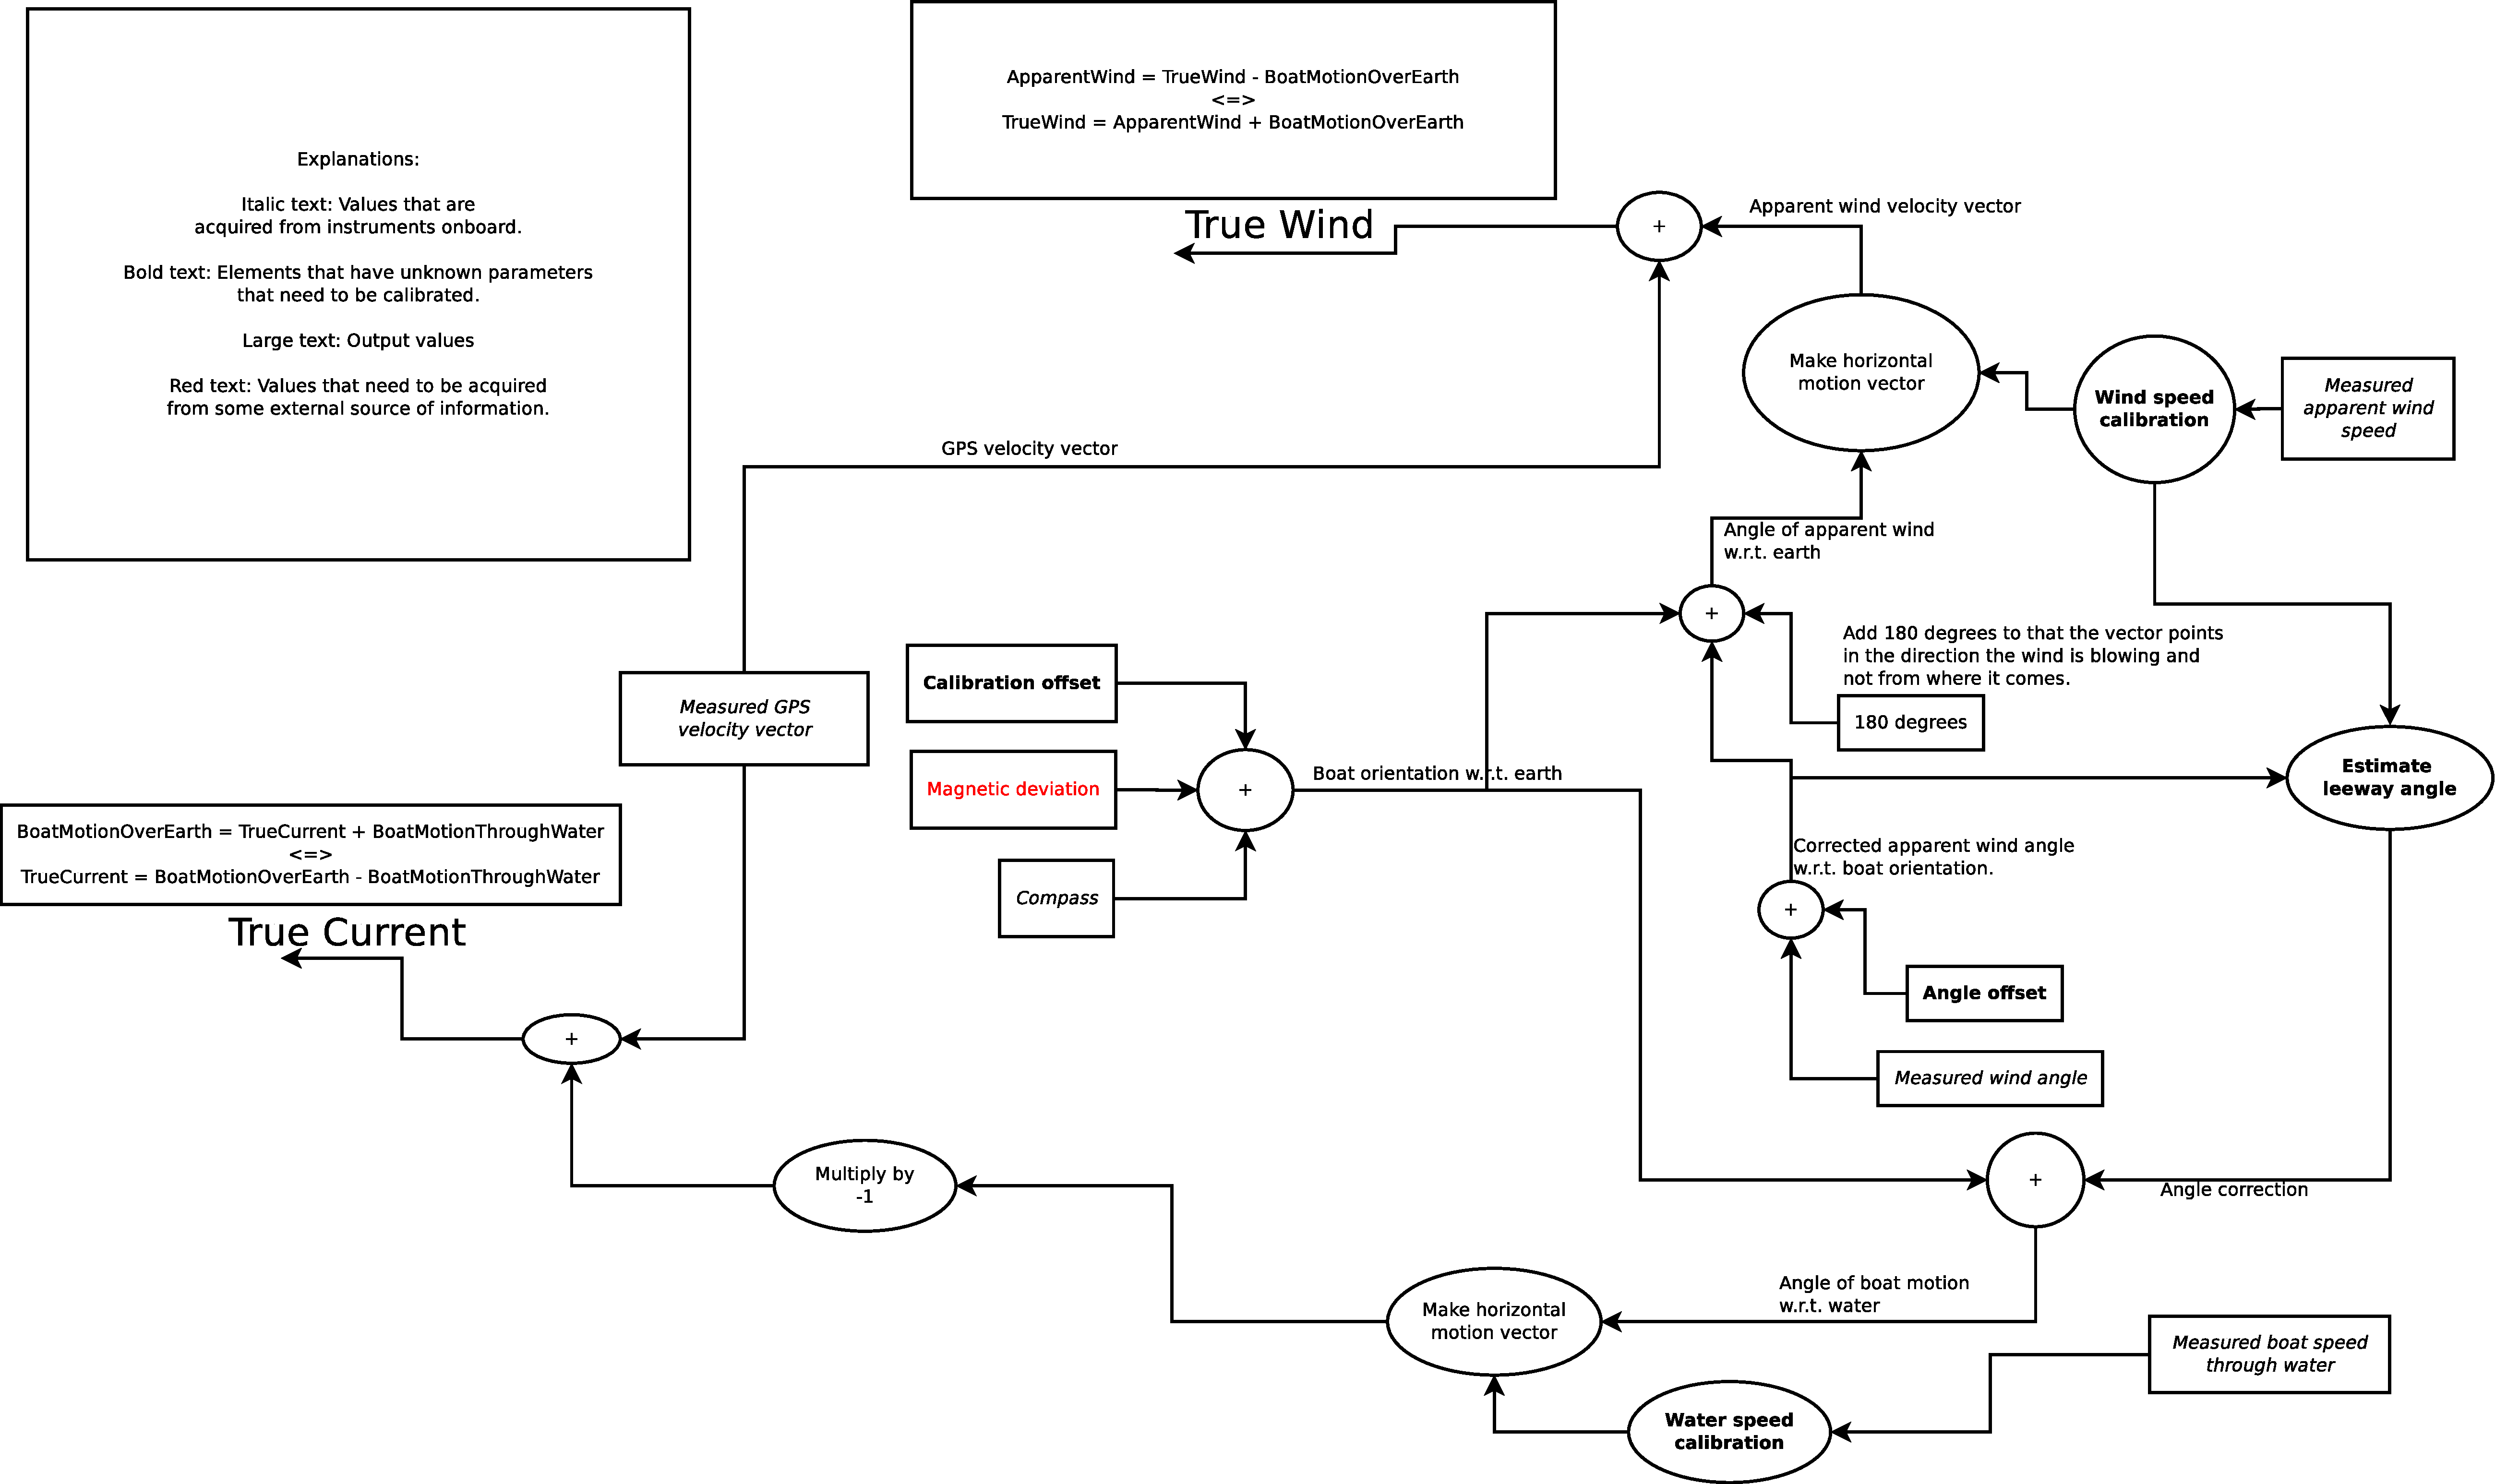
\includegraphics[width=\textwidth]{simplecalib.pdf}
\caption{Diagram illustrating how local true wind and current can be estimated from measurements coming from instruments on a boat.}
\label{fig:calib}
\end{figure}

We optimize the calibration parameters at densely sampled times $t_i \in \realnumber$ with $i$ in $1 \ldots N$. Typically, the difference between $t_i$ and $t_{i+1}$ could be a few seconds. We also introduce binary membership variables $a_i, b_i \in \{0, 1\}$ that determine whether or not to enforce wind or current stability, respectively.

With $\realvec{X} \in \realnumber^n$ being the calibration parameters and $\realvec{A} = (a_1, ..., a_N) \in \{0, 1\}^N$, $\realvec{B} = (b_1, ..., b_N) \in \{0, 1\}^N$ being the binary membership variables, we solve this optimization problem:
\begin{displaymath}
\underset{\realvec{X} \in \realnumber^n, \realvec{A} \in \{0, 1\}^N, \realvec{B} \in \{0, 1\}^N}{\text{Minimize}} \qquad \sum_{i = 1}^N  a_i\left(  \quality{w}^2\norm{\timederivative{\realvec{w}}(t_i, \realvec{X})}^2 - \norm{\timederivative{\realvec{g}}(t_i)} \right)
+ b_i\left( \quality{c}^2\norm{\timederivative{\realvec{c}}(t_i, \realvec{X})}^2 - \norm{\timederivative{\realvec{g}}(t_i)}\right) \, .
\end{displaymath}
The objective function tries to minimize the derivatives of estimated true wind and current whenever the corresponding membership variable is 1. The purpose of the derivative of the GPS velocity is to encourage the inclusion of measurements for which rapid changes in the velocity of the boat takes place. If it were excluded from the objective function, all membership variables could trivially be set to 0 and the result would be useless. The quality parameters $\quality{w}$ and $\quality{c}$ control how well we require the measurements to fit in order for them to directly influence the calibrated parameters.

It is easy to see that given a parameter vector $\realvec{X}$, the membership variables can be estimated directly for each term indidually by just looking at its sign. This lets us eliminate the membership variables, and we get the problem:
\begin{displaymath}
\underset{\realvec{X} \in \realnumber^n}{\text{Minimize}} \qquad \sum_{i = 1}^N  \minfun\left(0, \quality{w}^2\norm{\timederivative{\realvec{w}}(t_i, \realvec{X})}^2 - \norm{\timederivative{\realvec{g}}(t_i)}\right)
+ \minfun\left(0, \quality{c}^2\norm{\timederivative{\realvec{c}}(t_i, \realvec{X})}^2 - \norm{\timederivative{\realvec{g}}(t_i)}\right) \, .
\end{displaymath}
Furthermore, by adding a constant to the objective function it can be rewritten as a sum of truncated quadratic functions:
\begin{displaymath}
\underset{\realvec{X} \in \realnumber^n}{\text{Minimize}} \qquad \sum_{i = 1}^N  \minfun\left(\norm{\timederivative{\realvec{g}}(t_i)}, \quality{w}^2\norm{\timederivative{\realvec{w}}(t_i, \realvec{X})}^2\right)
+ \minfun\left(\norm{\timederivative{\realvec{g}}(t_i)}, \quality{c}^2\norm{\timederivative{\realvec{c}}(t_i, \realvec{X})}^2\right) \; .
\end{displaymath}
This type of cost function is used for robust fitting purposes, where we want to identify outliers. In our case, we can define a robust cost:
\begin{displaymath}
r_0(x, \sigma) =
\left\{
\begin{array}{ll}
  x^2 & |x| \leqslant \sigma \\
  \sigma^2 & \sigma < |x|
\end{array}
\right. \; ,
\end{displaymath}
where $\sigma$ is a threshold that separates inliers from outliers. This lets us rewrite the optimization problem to the form
\begin{displaymath}
\underset{\realvec{X} \in \realnumber^n}{\text{Minimize}} \qquad \sum_{i = 1}^N 
\quality{w}^2r_0\left(\norm{\timederivative{\realvec{w}}(t_i, \realvec{X})}, \sqrt{\frac{\norm{\timederivative{\realvec{g}}(t_i)}}{\quality{w}^2}}\right) + 
\quality{c}^2r_0\left(\norm{\timederivative{\realvec{c}}(t_i, \realvec{X})}, \sqrt{\frac{\norm{\timederivative{\realvec{g}}(t_i)}}{\quality{c}^2}}\right)\; .
\end{displaymath}
Although it looks more elaborate, it is now straight forward to replace the robust cost function $r_0$ by some other cost function, such as the Geman-McClure cost function
\begin{displaymath}
r_1(x, \sigma) = \frac{x^2\sigma^2}{x^2 + \sigma^2}\,,
\end{displaymath}
that has a similar but smoother shape which might work better with iterative solvers such as Levenberg-Marquardt. This cost function also has the advantage that its derivative is zero in just a few discrete points, meaning that an optimization algorithm can converge to a local optimum without a careful initialization.
\subsection{Parameter tuning}
As previously discussed, we have one parameter $\quality{w}$ to control wind fitness quality and one paramater $\quality{c}$ for controlling current fitness quality. Typically, water has more inertia than air and we would expect the wind related terms in the objective function to fluctuate much more than the current related ones. Having a common quality parameter $q = \quality{w} = \quality{c}$ might lead to almost all current related terms to be inliers whereas many wind related terms might be outliers, ultimately leading to poor results. By having seperate quality parameters, we would expect a better balance between the wind and current related contribution to the calibration.

One possible way to initialize the quality parameters would be to assign fixed values to them. This, however, could lead to very few inliers or too many inliers, depending on the underlying data. Another strategy would be, given the initial calibration parameters assuming no distortion of the raw measurements, to adjust the quality parameters so that a fixed number of the measurements become inliers.

A more sophisticated way of tuning the quality parameters would be to adjust the wind and current parameters using cross validation, to minimize the difference in true computed wind and current, respectively, over different data splits.
\section{Implementation}
The derivatives in the objective function are estimated using finite differences. Differentiation increases noise, so the signals over which we optimize must be denoised before they can be used in the optimization, e.g. using second order Total Variation (TV) denoising which tends to produce piecewise constant derivatives of the signals.

We minimize the last form of the objective function, expressed in terms of robust cost functions. If we use the $r_0$ robust cost, the objective function becomes nonsmooth in some points, but this is usually not a problem. If we want to be sure to have a smooth objective function, we can replace the $r_0$ cost function by a smooth one, such as $r_1$.

\section{Discussion}
It would be nice to investigate the following:
\begin{itemize}
\item How stable the calibrated values are as the quality parameters are varied.
\item How stable the calibrated values are over different splits (cross-validation). Compare the true winds and currents.
\item Add corruptions to the measurements to see if these corruptions are recovered in the calibration parameters.
\item Compare recovered true winds and currents with measures taken from another nearby boat.
\end{itemize}

\end{document}


